\chapter{Experiments and Evaluation}\label{ch:experiments-and-evaluation}
In this chapter the experimental procedure is described in detail, and the evaluation
including the quantitative results are presented.


\section{Experimental Setup}\label{sec:experimental-setup}
I implemented the PPO algorithm in Python using PyTorch for the implementation of the
neural networks and the optimization~\cite{NEURIPS2019_9015}.
For the environments I used the openAI gym in combination with PyBulletEnv for an open-source implementation of the simulation
for the robotic environments~\cite{brockman2016openai,benelot2018}.
Further, I employed Stablebaselines3 for the normalization of the environment~\cite{stable-baselines3}.
In particular, I normalized both the state space and rewards.
The two considered environments are Pendulum-v0 and AntPyBulletEnv-v0.
Figure~\ref{fig:envs} illustrates the environments.
\begin{figure}[t]
    \centering
    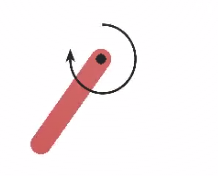
\includegraphics[width=0.25\textwidth]{images/presentation/pendulum-v0.png}
    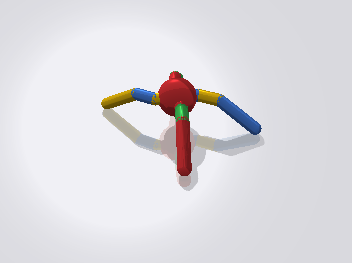
\includegraphics[width=0.35\textwidth]{images/presentation/ant.png}
    \caption{Rendering of the environments. Pendulum-v0 on the left and AntPyBulletEnv-v0 on the right.}
    \label{fig:envs}
\end{figure}
The training was conducted on an AMD Ryzen 2700X CPU for a total of 1 million training steps.
The policy and value function are modeled by separate neural networks respectively.
The architecture is presented in Section~\ref{sec:proximal-policy-optimization}.
Table~\ref{tab:hyp} presents the hyperparameters used during training.
\begin{table}[t]
    \centering
    \begin{tabular}{c|c | c}
        \toprule
        Hyperparameter & Pendulum-v0 &  AntPyBulletEnv-v0\\
        \midrule
        $\varepsilon$-clip & 0.2 & 0.2\\
        $\gamma$ & 0.99 & 0.99\\
        $\sigma$ & 0.5 & 0.1\\
        $N$ & 2048 & 2048\\
        $T$ & 200 & 32\\
        $K$ & 10 & 10\\
        numeric stability & $1\cdot 10^{-10}$ & $1\cdot 10^{-10}$\\
        learning rate & $2\cdot 10^{-4}$ & $2.5\cdot 10^{-4}$\\
        \bottomrule
    \end{tabular}
    \caption{Hyperparameters used during training.}
    \label{tab:hyp}
\end{table}
The naming is in accordance with Algorithm~\ref{alg:ppo}.
Additionally, $\sigma$ refers to the variance used to initialize the covariance matrix used in the multivariate gaussian
to sample an action from the mean-value provided by the policy network.
To ensure numeric stability when normalizing the advantage function estimates the shown hyperparameter is added
during normalization.
The learning rate is used for both the value function and policy network.

\section{Evaluation}\label{sec:evaluation}
Section~\ref{subsec:pendulum-v0} presents the results on the comparatively simple Pendulum-v0 environment.
Section~\ref{subsec:antpybulletenv-v0} shows the behaviour of the algorithm on a more complex environment.

\subsection{Pendulum-v0}\label{subsec:pendulum-v0}
The Pendulum-v0 environment is considered one of the easier environments.
This is in part due to the low dimensionality of the state space with only three dimensions, and a single control signal.
Both the state space, and the action space are continuous.
Figure~\ref{fig:training_pendulum} displays the progress during training.
\begin{figure}[t]
    \centering
    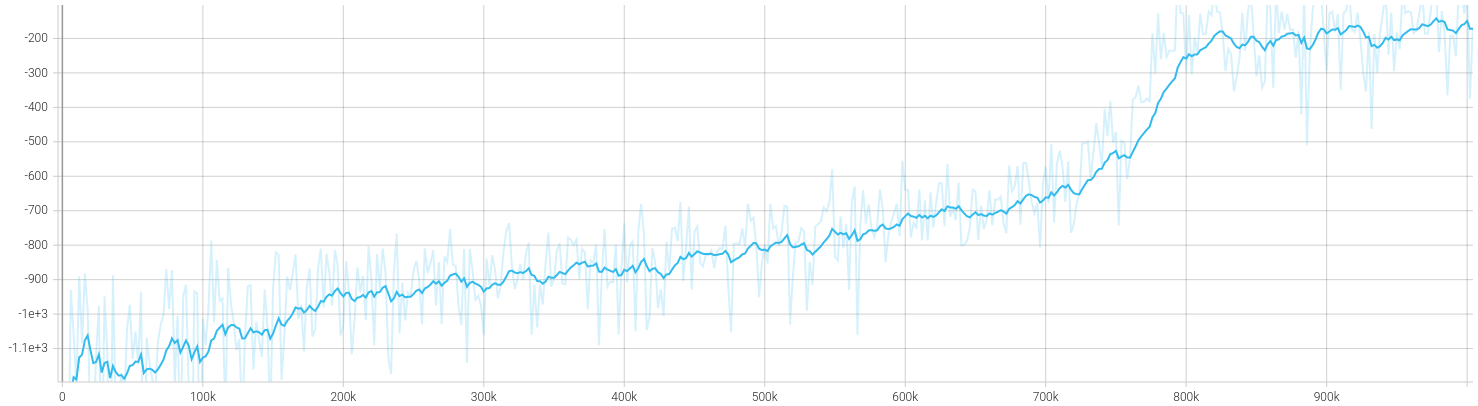
\includegraphics[width=1\textwidth]{images/presentation/train_pendulum.png}
    \caption{Training process of my implementation of the PPO algorithm on the Pendulum-v0 environment.}
    \label{fig:training_pendulum}
\end{figure}
The y-axis shows the average episodic return throughout the training process, the x-axis denotes the time step.
To obtain the results three runs on random seeds are considered, and their results are averaged.
As shown in Figure~\ref{fig:training_pendulum} the model achieves an average episodic return of around $-175$.

\subsection{AntPyBulletEnv-v0}\label{subsec:antpybulletenv-v0}
The AntPyBulletEnv-v0 environment is considered significantly more complex than the Pendulum-v0.
This is demonstrated by the increased state space dimension of $28$, and an action space dimension of $8$.
Again, action space and state space are continuous.
Figure~\ref{fig:training_ant} displays the training process on the AntPyBulletEnv-v0 environment.
The y-axis shows the average episodic return during training, the x-axis denotes the time step.
Note that the average episodic return is gathered during training thus, it is normalized to the average episodic
length and therefore not the same as the results presented in the following.
\begin{figure}[t]
    \centering
    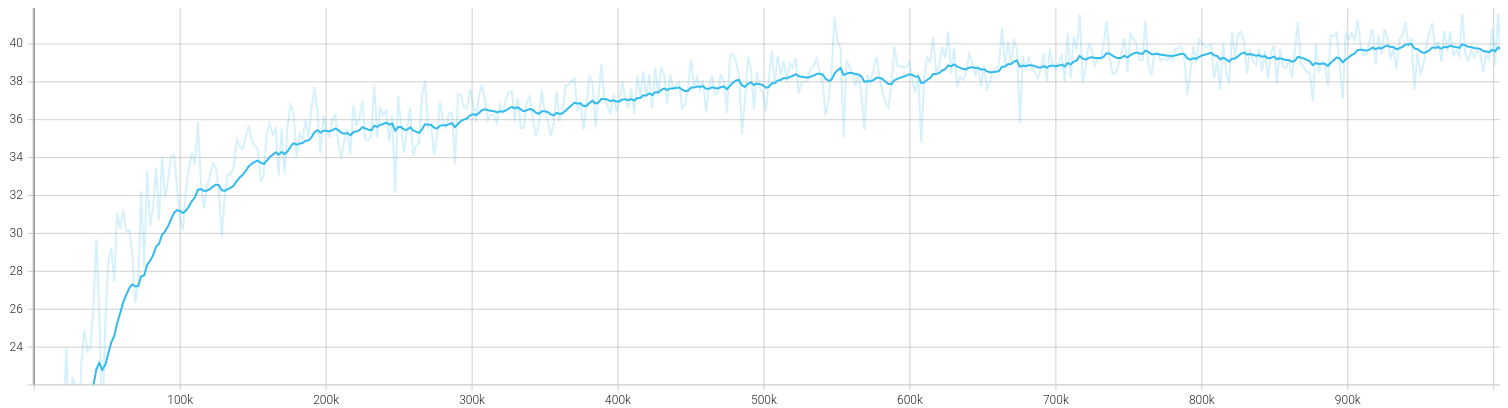
\includegraphics[width=\textwidth]{images/presentation/ant_train.png}
    \caption{Training process of my implementation of the PPO algorithm on the AntPyBulletEnv-v0 environment.}
    \label{fig:training_ant}
\end{figure}
Further, Figure~\ref{fig:loss} shows the loss function of the policy network and value function network
respectively.
The results are obtained by averaging three runs on random seeds.
I was however unable to replicate the average episodic return achieved during training in the evaluation.
I was unable to identify my error and therefore assume an implementation error in the evaluation code.
However, considering the fixed episodic length of $32$ during training and an episodic length of $1000$ during evaluation
an average return of around $1250$ would be expected.
Note that I corrected the results such that the influence of extremely short sequences does not influence the final score.
\begin{figure}[t]
    \centering
    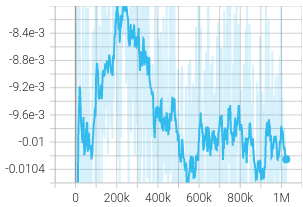
\includegraphics[width=0.3\textwidth]{images/presentation/ant_loss_policy.png}
    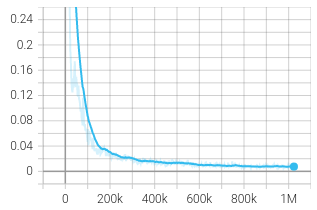
\includegraphics[width=0.3\textwidth]{images/presentation/ant_loss_value.png}
    \caption{Loss function values of the policy network on the left and the value function network on the right.}
    \label{fig:loss}
\end{figure}


